%  TODO: add the environement part,
%  TODO: add perspective 

\section{Experimental Guidelines}\label{sec:guidelines}
To summarize our experiments, we provide some experimental guidelines in Table~\ref{table:guidelines}, based on the multiple experiments and analysis we did.
These guidelines constitute a set of minimal requirements or best practices, depending on the workload and the criticality of the energy measurement precision.
It therefore intends to help practitioners in taming the energy variation on the selected CPU, and conduct the experiments with the least variations.

\begin{table}[h!]
    \centering
    \caption{Experimental Guidelines for Energy Variations}
    \small
    \begin{tabular}{|p{4.7cm}|c|c|}
        \hline
        \textbf{Guideline}                                                                                                                                                & \textbf{Load} & \textbf{Gain}     \\
        \hline
        \hline
        Use a low TDP CPU                                                                                                                                                 & Low \& medium & Up to $3\times$   \\
        \hline
        Disable the CPU C-states                                                                                                                                          & Low           & Up to $6\times$   \\
        \hline
        Use the least of sockets in a case of multiple CPU                                                                                                                & Medium        & Up to $30\times$  \\
        \hline
        Avoid the usage of hyper-threading whenever possible                                                                                                              & Medium        & Up to $5\times$   \\
        \hline
        Avoid rebooting the machine between tests                                                                                                                         & High          & Up to $1.5\times$ \\
        \hline
        Do not relate to the machine idle variation to isolate a test EC, the CPU/OS changes its behavior when a test is running and can exhibit less variation than idle & Any           & ---               \\
        \hline
        Rather focus the optimization efforts on the system under test than the OS                                                                                        & Any           & ---               \\
        \hline
        Execute all the similar and comparable experiments on a same machine. Identical machines can exhibit many differences regarding their energy behavior             & Any           & Up to $1.3\times$ \\
        \hline
    \end{tabular}
    \label{table:guidelines}
\end{table}

Table~\ref{table:guidelines} gives a proper understanding of known factors, like the C-states and its variation reduction at low workloads.
However, it also lists some new factors that we identified along the analysis we conducted in Section, such as the results related to the OS or the reboot mode.
Some of the guidelines are more useful/efficient for specific workloads, as showed in our experiments.
Thus, qualifying the workload before conducting the experiments can help in choosing the proper guidelines to apply.
Other studied factors are not been mentioned in the guidelines, like the Turbo~Boost or the Speculative execution, due to the small effect that has been observed in our study.

In order to validate the accuracy of our guidelines among a varied set of benchmarks on one hand, and their effect on the variation between identical machines on the other hand, we ran seven experiments with benchmarks and real applications on a set of four identical nodes from the cluster \textsf{Dahu}, before (\textsf{normal} mode where everything is left to default and to the charge of the OS) and after (\textsf{optimized}) applying our guidelines.
Half of these experiments has been performed at a 50\,\% workload and the other half on single process jobs.
The choice of these two workloads is related to the optimization guidelines that are mainly effective at low and medium workloads.
We note that we used the cluster \textsf{Dahu} over \textsf{Ecotype} to highlight the guidelines effect on the nodes where the variation is susceptible to be higher.

\begin{figure*}%[!htb]
    \center{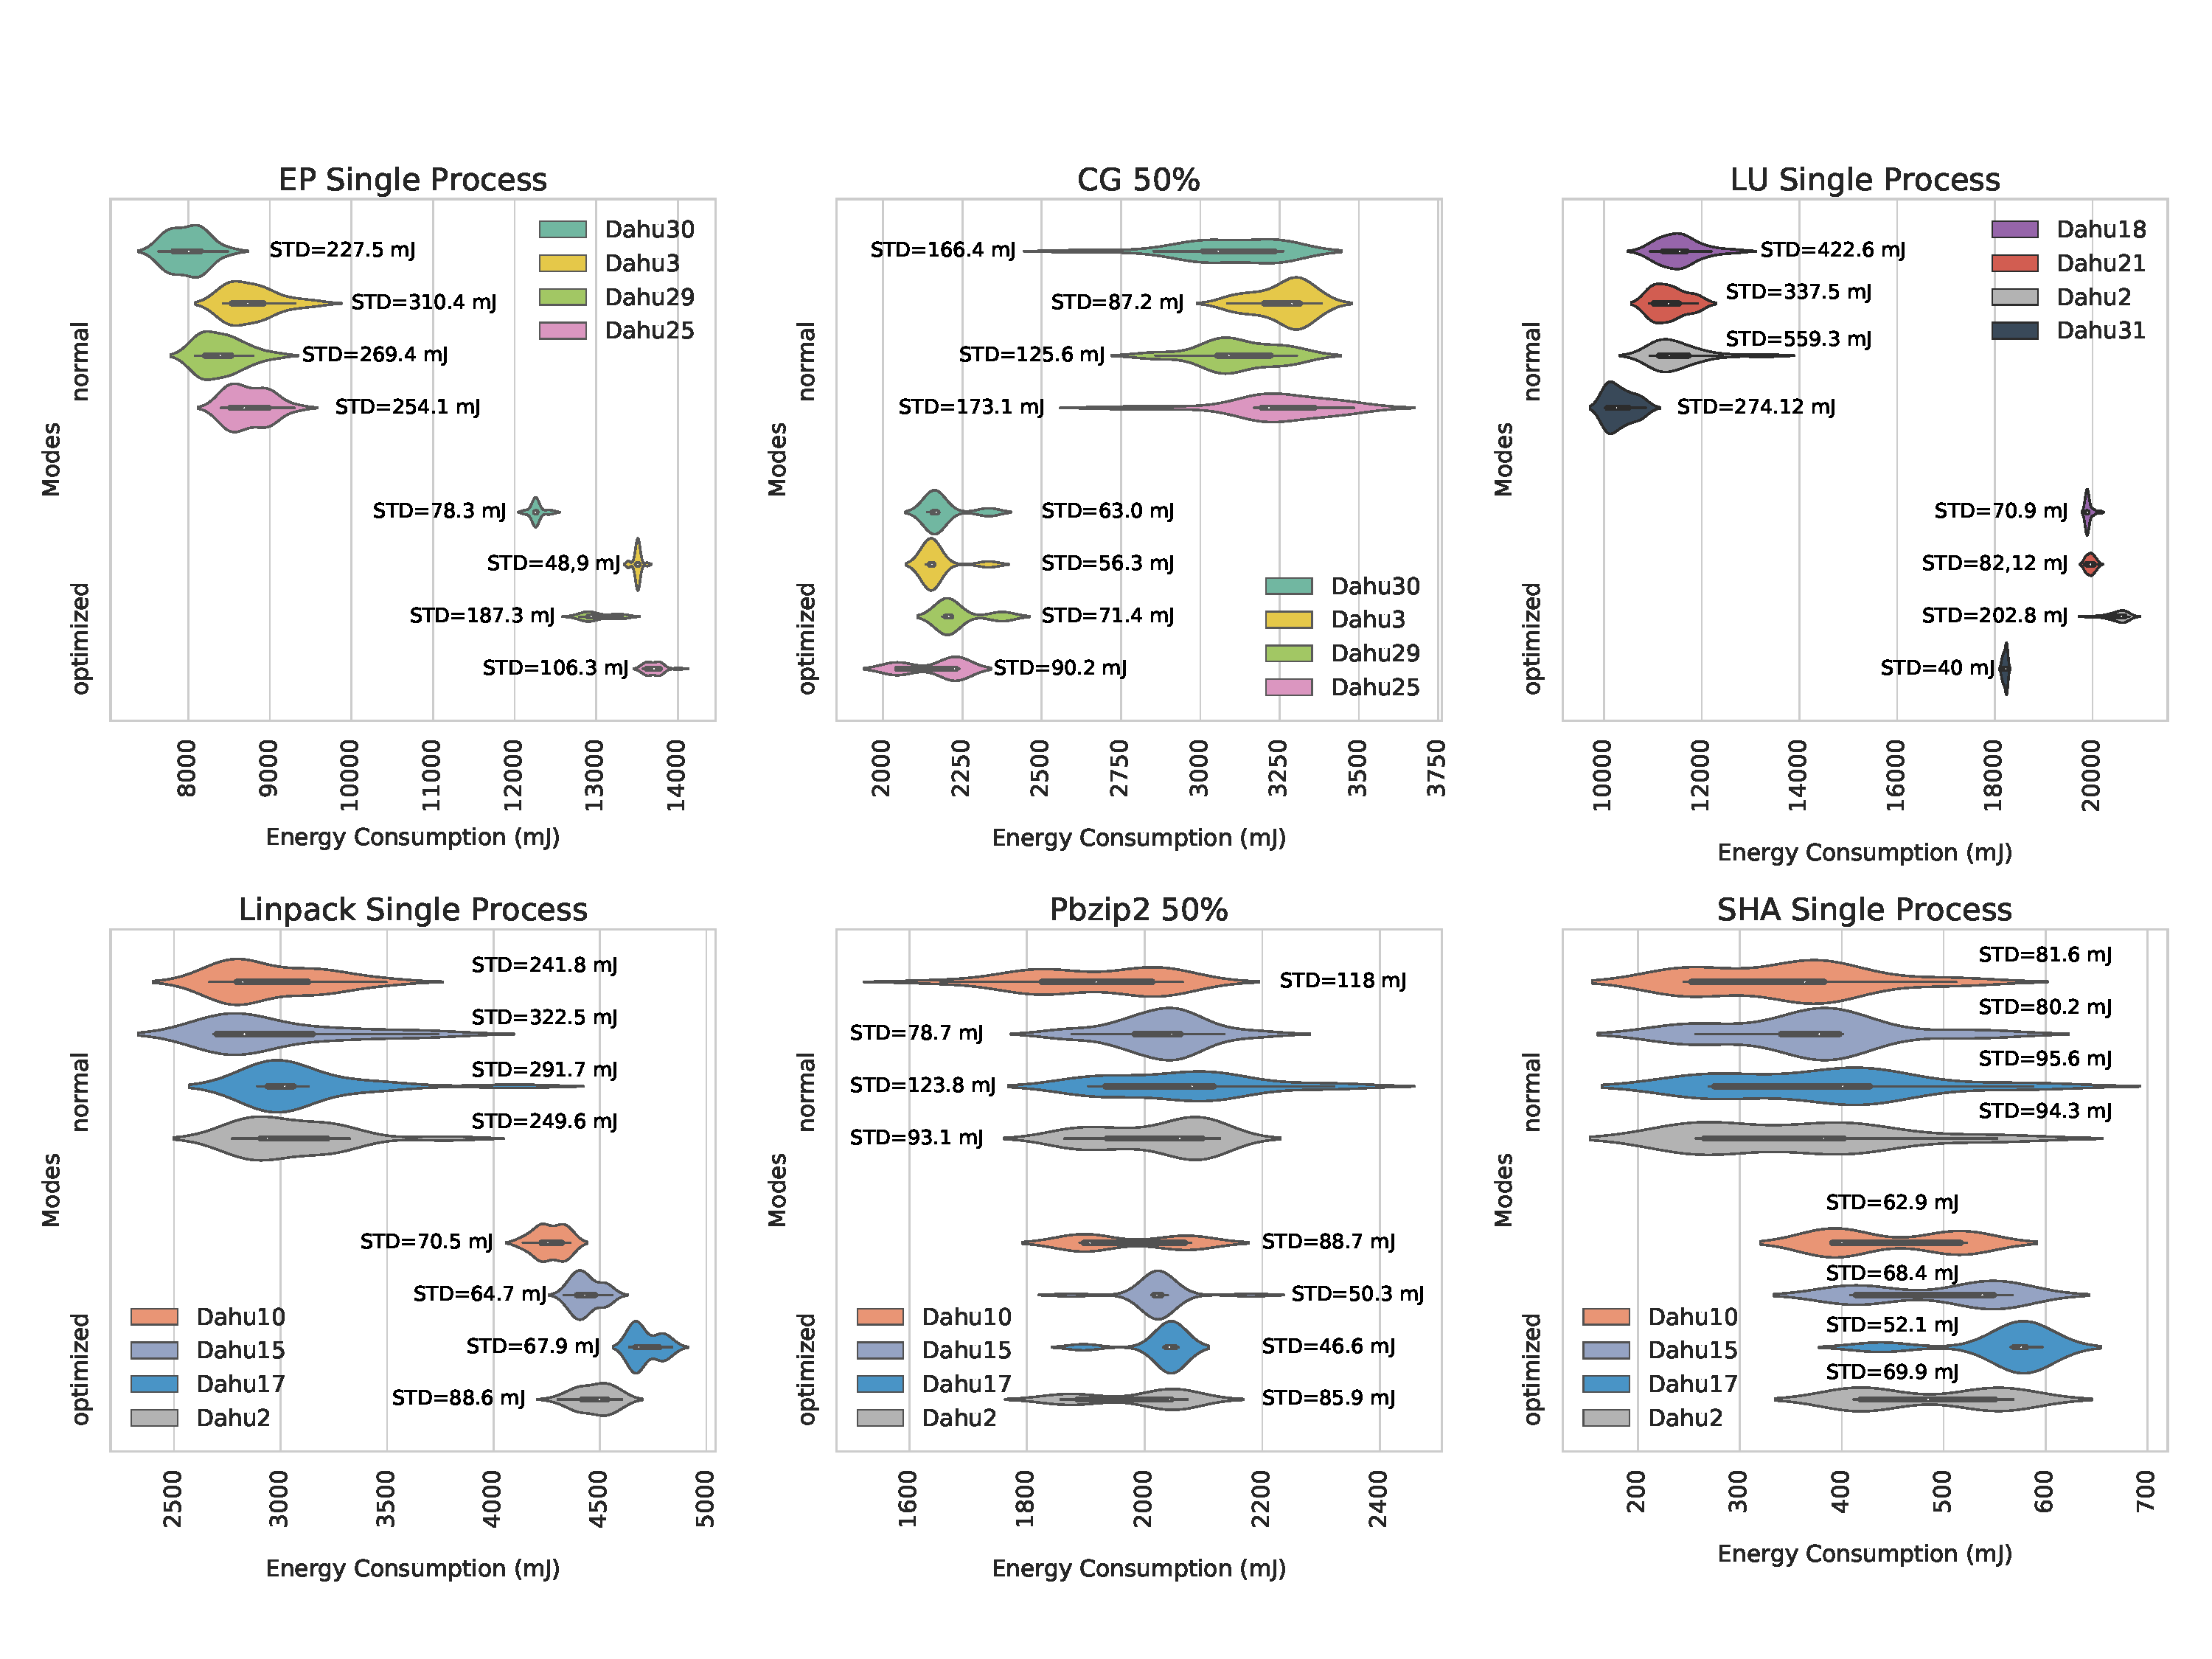
\includegraphics[width=\linewidth]{imgs/all}}
    \caption{Energy variation comparison with/without applying our guidelines}\label{fig:optimized}
\end{figure*}

\begin{figure}%[!htb]
    \center{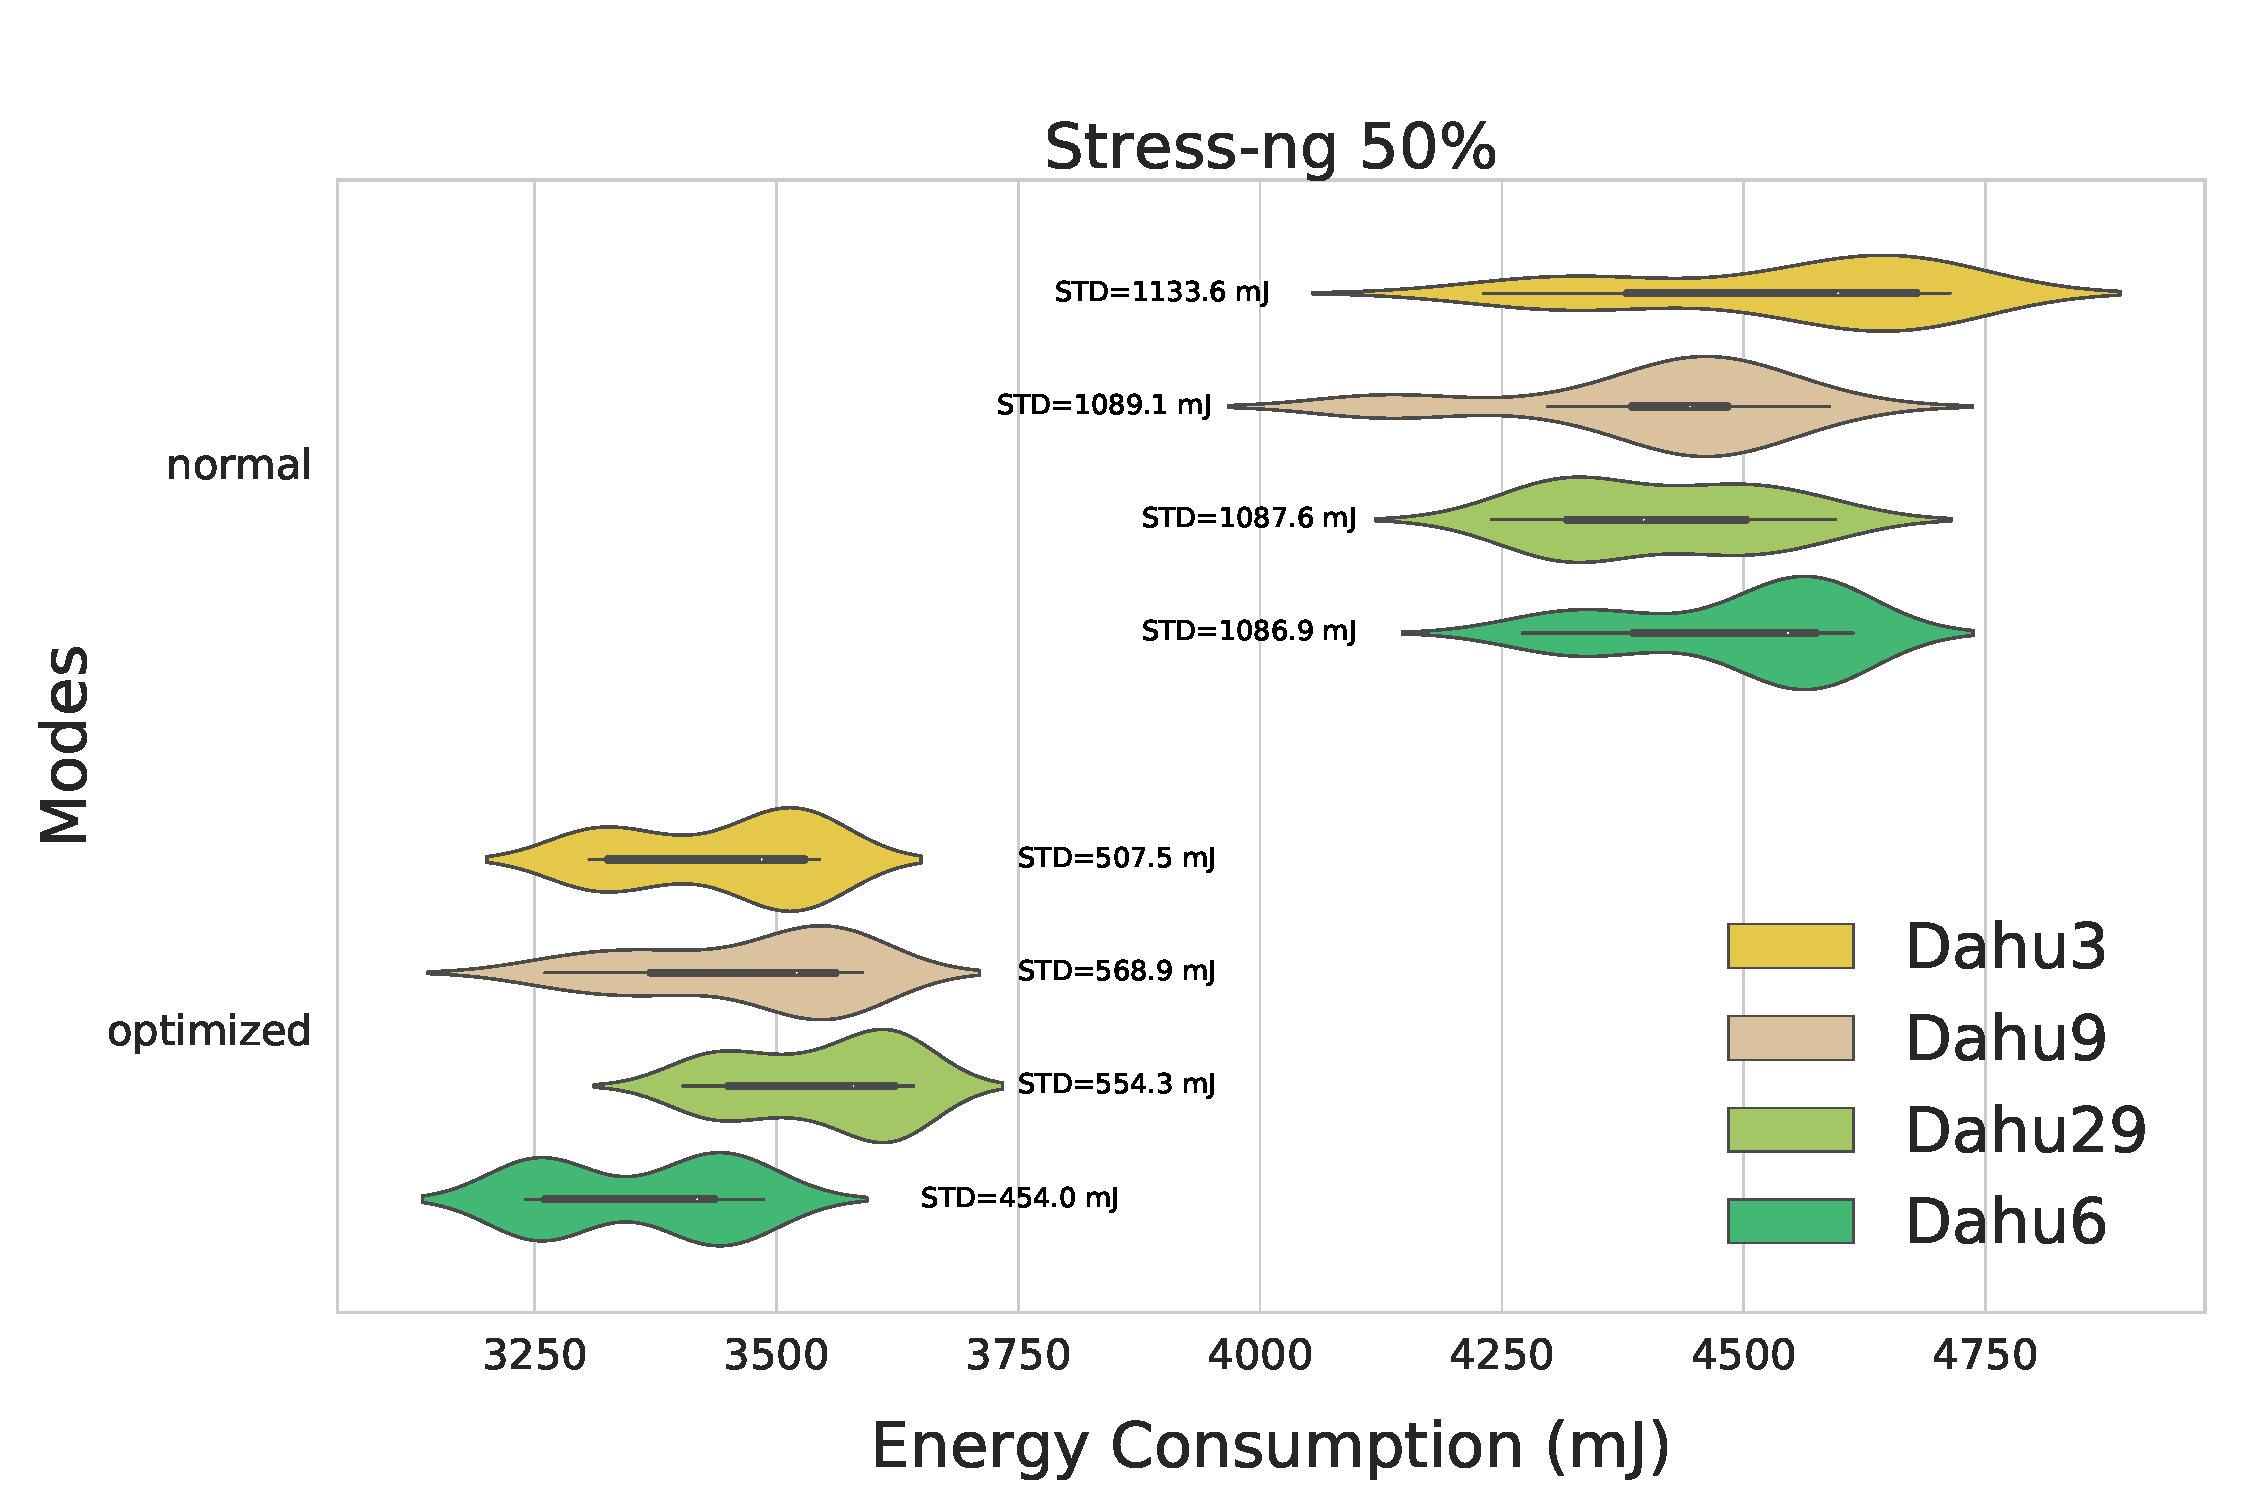
\includegraphics[width=.9\linewidth]{imgs/stressng}}
    \caption{Energy variation comparison with/without applying our guidelines for \textsc{Stress-NG}}\label{fig:stress}
\end{figure}

Figure~\ref{fig:optimized} and~\ref{fig:stress} highlight the improvement brought by the adoption of our guidelines.
They demonstrate the intra-node STD reduction at low and medium workloads for all the benchmarks used at different levels.
Concretely, for low workloads, the energy variation is 2--6 times lower after applying the optimization guidelines for the benchmarks \textsf{LU} and \textsf{EP}, as well as \textsc{Linpack}, while it is 1.2--1.8 times better for \texttt{Sha256}.
For this workload, the overall energy consumption after optimization can be up to 80\,\% higher due to disabling the C-states to keep all the unused cores at a high power consumption state ($Mean_{LU-normal-Dahu2}=11,500 mJ$, $Mean_{LU-optimized-Dahu2}=20,508 mJ$).
For medium workloads, the STD, and thus variation, is up to 100\,\% better for the benchmark \textsf{CG}, 20--150\,\% better for the \texttt{pbzip2} application and up to 100\% for \textsc{Stress-NG}.
We note that the optimized version consumes less energy thanks to an appropriate core pinning method.

Figures~\ref{fig:optimized} and~\ref{fig:stress} also highlight that applying the guidelines does not reduce the inter-nodes variation in all the cases.
This variation can be up to 30\,\% in modern CPU~\cite{wang_experimental_nodate}.
However, taming the intra-node variation is a good strategy to identify more relevant mediums and medians, and then perform accurate comparisons between the nodes variation.
Even though, using the same node is always better, to avoid the extra inter-nodes variation and thus improve the stability of measurements.

\section{Threats to Validity}\label{sec:threats}
A number of issues affect the validity of our work.
For most of our experiments, we used the Intel RAPL tool, which has evolved along Intel CPU generations to be known as one of the most accurate tools for modern CPU, but still adds an important overhead if we adopt a sampling at high frequency.
The other fine-grained tool we used for measurements is \textsc{PowerAPI}.
It allows to measure the energy consumption at the granularity of a process or a Cgroup by dividing the RAPL global energy over the running processes using a power model.
The usage of \textsc{PowerAPI} adds an error margin because of the power model built over RAPL.
The RAPL tool mainly measures the CPU and DRAM energy consumption.
However, even running CPU/RAM intensive benchmarks would keep a degree on uncertainty concerning the hard disk and networking energy consumption.
In addition, the operating system adds a layer of confusion and uncertainty.

The Intel CPU chip manufacturing process and the materials micro-heterogeneity is one of the biggest issues, as we cannot track or justify some of the energy variation between identical CPU or cores.
These CPU/cores might handle frequencies and temperature differently and behave consequently.
This hardware heterogeneity also makes reproduction complex and requires the usage of the same nodes on the cluster with the same OS.

% A more subtle issue may arise due to the values of the measurements that we achieved.
% In fact, the energy measures are quite small, and iterations may be taking a few milliseconds more or less to run.
% A thing we cannot measure using our measurement tools.
% How generalizable are our results? As a set of energy variation optimization guidelines, we argue that our results applied on most of the modern Intel CPU.
% However, using and comparing identical CPU is still tricky and is very dependent to chips.


\section{Conclusion}\label{sec:conclusion}
In this paper, we conducted an empirical study of controllable factors that can increase the energy variations on platforms with some of the latest CPU, and for several workloads.
We provide a set of guidelines that can be implemented and tuned (through the OS GRUB for example), especially with the new data centers isolation trend and the cloud usage, even for scientific and R\&D purposes.
Our guidelines aim at helping the user in reducing the CPU energy variation during systems benchmarking, and conduct more stable experiments when the variation is critical.
For example, when comparing the energy consumption of two versions of an algorithm or a software system, where the difference can be tight and need to be measured accurately.

Overall, our results are not intended to nullify the variability of the CPU, as some of this variability is related to the chip manufacturing process and its thermal behavior.
The aim of our work is to be able to tame and mitigate this variability along controlled experiments.
We studied some previously discussed aspects on some recent CPU, considered new factors that have not been deeply analyzed to the best of our knowledge, and constituted a set of guidelines to achieve the variability mitigating purpose.
Some of these factors, like the C-states usage, can reduce the energy variation up to 500\,\% at low workloads, while choosing the wrong cores/PU strategy can cause up to $30\times$ more variability.

We believe that our approach can also be used to study/discover other potential variability factors, and extend our results to alternative CPU generations/brands.
Most importantly, this should motivate future works on creating a better knowledge on the variability due to CPU manufacturing process and other factors.


\section{Perspectives}
By the end of this study we have gathered enought guidelines to make the tests more reproducible, accurate.
We created a set of new tests named \textbf{energy tests} which are more similar to performance tests. Thanks to the work of two interns [ mamadou and adrien] we created a CI/CD plateform to measure the energy consumption of Java projects and we could track the evolution of the this energy accross different stages of the project.
In the figure below we see an example of this plugin.
For more details please visit the gitlab repository ... add link.

\begin{figure}%[!htb]
    \center{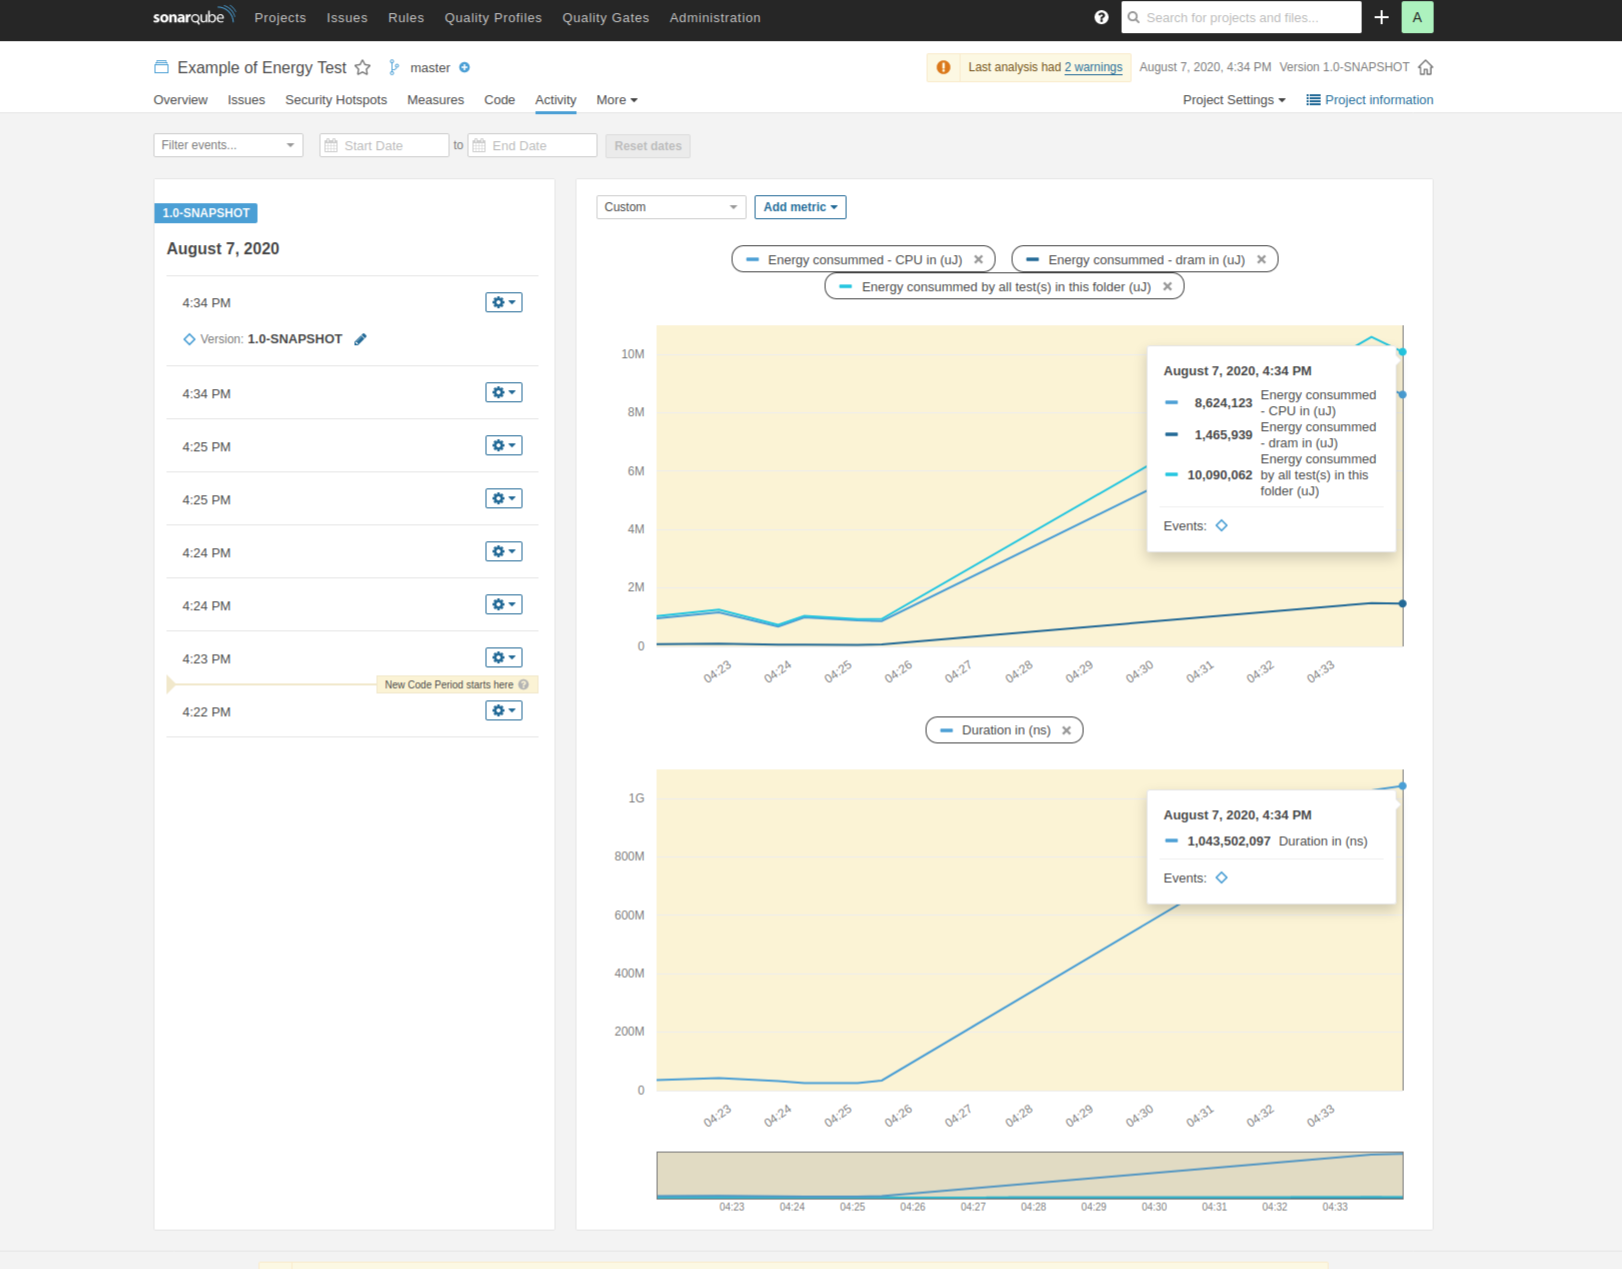
\includegraphics[width=.9\linewidth]{imgs/JunitSonarplugin}}
    \caption{Example of the Junit Sonar Plugin}\label{fig:sonar_plugin}
\end{figure}

% However for them to be more representatives we wanted to simulate the production enviromenet.
%% should i add  the thing about green faas ? 
%% same about what we have done with python workers and lazy ? basically just a graph 
